\documentclass[12pt,a4paper]{article}
\usepackage[utf8]{inputenc}
\usepackage[T2A]{fontenc}
\usepackage[russian]{babel}
\usepackage{amsmath,amssymb}
\usepackage{graphicx}
\usepackage{float}
\usepackage{caption}
\usepackage{booktabs}
\usepackage{array}
\usepackage{geometry}
\geometry{left=2cm,right=2cm,top=2cm,bottom=2cm}
\usepackage{siunitx}
\sisetup{output-decimal-marker={,}}
\usepackage{indentfirst}
\usepackage{setspace}
\onehalfspacing

\begin{document}

% Титульная страница
\begin{titlepage}
    \centering
    \vspace*{2cm}
    {\Large Московский физико-технический институт\\[0.5ex]
    (национальный исследовательский университет)\par}
    \vspace{1cm}
    {\large Кафедра общей физики\par}
    \vspace{2cm}
    {\LARGE \textbf{Лабораторная работа № 1.3.3}\par}
    \vspace{1cm}
    {\huge \textbf{Измерение вязкости воздуха\\ по течению в тонких трубках}\par}
    \vspace{3cm}
    \begin{flushright}
        \large
        Студент: \textit{Осипов Максим}\\
        Группа: Б03-504\\
        Дата выполнения: 15.04.2026
    \end{flushright}
    \vfill
    Долгопрудный, 2026
\end{titlepage}

% Аннотация
\section*{Аннотация}
\textbf{Цель работы:} экспериментальное исследование течения воздуха в тонких трубках при различных числах Рейнольдса, определение области применимости закона Пуазейля и вычисление коэффициента вязкости воздуха.

\textbf{Оборудование:} система подачи воздуха (компрессор), газовый счётчик барабанного типа ГСБ-400, спиртовой микроманометр с регулируемым наклоном, набор трубок диаметрами \qty{3.0}{мм}, \qty{4.1}{мм}, \qty{5.2}{мм}, секундомер.


\section{Теоретические сведения}

\subsection{Закон Ньютона для вязкого трения}
Сила внутреннего трения между слоями жидкости или газа описывается законом Ньютона:
\begin{equation}
    \tau_{xy} = -\eta \frac{\partial v_x}{\partial y},
\end{equation}
где $\eta$ — коэффициент динамической вязкости, $\tau_{xy}$ — касательное напряжение.

\subsection{Число Рейнольдса и режимы течения}
Характер течения определяется безразмерным числом Рейнольдса:
\begin{equation}
    \mathrm{Re} = \frac{\rho \bar{v} d}{\eta},
\end{equation}
где $\rho$ — плотность среды, $\bar{v}$ — средняя скорость потока, $d$ — диаметр трубы.
\begin{itemize}
    \item При $\mathrm{Re} \lesssim 10^3$ течение ламинарное (слоистое, устойчивое);
    \item При $\mathrm{Re} \gtrsim 10^3$ течение становится турбулентным (вихревое, с флуктуациями).
\end{itemize}

\subsection{Течение Пуазейля (ламинарный режим)}
Для установившегося ламинарного течения в прямой трубе круглого сечения:
\begin{itemize}
    \item Давление линейно убывает вдоль трубы: $P(x) = P_0 - \frac{\Delta P}{L} x$;
    \item Профиль скорости параболический: $v(r) = \frac{\Delta P}{4\eta L}(R^2 - r^2)$;
    \item Объёмный расход описывается формулой Пуазейля:
    \begin{equation}
        Q = \frac{\pi R^4 \Delta P}{8 \eta L}.
    \end{equation}
\end{itemize}

\subsection{Длина установления течения}
Профиль Пуазейля формируется не мгновенно, а на длине
\begin{equation}
    L_{\text{уст}} \approx 0.2 \cdot R \cdot \mathrm{Re}.
\end{equation}

\subsection{Вязкость газов}
На молекулярном уровне вязкость газа обусловлена переносом импульса при хаотическом движении молекул. Оценка:
\begin{equation}
    \eta \sim \frac{1}{3} \rho \bar{v}_{\text{тепл}} \lambda,
\end{equation}
где $\lambda$ — длина свободного пробега. Вязкость газа зависит от температуры, но практически не зависит от давления.

\subsection{Анализ размерностей (турбулентный режим)}
В турбулентном режиме строгое аналитическое решение отсутствует. Метод размерностей и модель турбулентной вязкости $\eta_{\text{турб}} \sim \rho \bar{v} R$ дают зависимость:
\begin{equation}
    Q \propto R^{5/2} \sqrt{\frac{\Delta P}{\rho L}} \quad \Rightarrow \quad Q \propto R^{2.5} \text{ при фиксированном } \frac{\Delta P}{L}.
\end{equation}

\section{Экспериментальная установка и методика измерений}

Схема установки приведена на рис.~\ref{fig:setup}. Воздух от компрессора через регулировочный кран поступает в газовый счётчик барабанного типа, затем проходит через одну из исследуемых трубок. Перепад давления на рабочем участке трубки измеряется спиртовым микроманометром с наклонной шкалой. Объёмный расход определяется по времени прохождения заданного объёма газа через счётчик.

\begin{figure}[H]
    \centering
    % Замените на реальный файл схемы
    
\includegraphics[width=0.8\textwidth]{установка.png}
    \caption{Схема экспериментальной установки.}
    \label{fig:setup}
\end{figure}

\subsection{Параметры окружающей среды и погрешности}
Температура воздуха $T = \qty{23.8}{\celsius}$, относительная влажность $\varphi = 28\%$, атмосферное давление $P_{\text{атм}} = \qty{98400}{\Pa}$. Плотность воздуха $\rho = \qty{1.165}{\kg/\m^3}$ (рассчитана по уравнению идеального газа).

Характеристики трубок и измерительных участков:
\begin{itemize}
    \item $d_1 = \qty{4.1}{\mm}$, длина участка $l = \qty{0.5}{\m}$;
    \item $d_2 = \qty{5.2}{\mm}$, $l = \qty{0.5}{\m}$;
    \item $d_3 = \qty{3.0}{\mm}$, $l = \qty{0.5}{\m}$.
\end{itemize}

Микроманометр: коэффициент наклона $K = 0.2$, цена деления \qty{0.2}{\mm вод.ст.}, пересчёт в паскали: $1\text{ дел} = \qty{1.961}{\Pa}$.

Погрешность измерения расхода $\varepsilon_Q \approx 1\%$, давления — $\sigma_{\Delta P} \approx \qty{1}{\Pa}$.

\section{Результаты измерений и обработка данных}

\subsection{Трубка диаметром $d_1 = \qty{4.1}{\mm}$}

В таблице~\ref{tab:d1_lam} представлены данные для ламинарного режима, в таблице~\ref{tab:d1_turb} — для турбулентного.

\begin{table}[H]
\centering
\caption{Ламинарный режим, $d_1 = \qty{4.1}{\mm}$.}
\label{tab:d1_lam}
\begin{tabular}{c c c c c c}
\toprule
№ & $\Delta t$, с & $\Delta V$, л & $Q$, л/с & $\Delta P$, дел & $\Delta P$, Па \\
\midrule
1 & 24.34 & 0.510 & 0.0205 & 13 & 25.5 \\
2 & 16.31 & 0.505 & 0.0309 & 20 & 39.2 \\
3 & 9.97  & 0.372 & 0.0373 & 25 & 49.0 \\
4 & 5.07  & 0.223 & 0.0440 & 30 & 58.8 \\
5 & 9.73  & 0.505 & 0.0519 & 35 & 68.6 \\
6 & 8.59  & 0.505 & 0.0588 & 40 & 78.4 \\
7 & 7.80  & 0.501 & 0.0642 & 44 & 86.3 \\
\bottomrule
\end{tabular}
\end{table}

\begin{table}[H]
\centering
\caption{Турбулентный режим, $d_1 = \qty{4.1}{\mm}$.}
\label{tab:d1_turb}
\begin{tabular}{c c c c c c}
\toprule
№ & $\Delta t$, с & $\Delta V$, л & $Q$, л/с & $\Delta P$, дел & $\Delta P$, Па \\
\midrule
1 & 6.43 & 0.499 & 0.0776 & 55 & 107.9 \\
2 & 5.63 & 0.505 & 0.0897 & 66 & 129.4 \\
3 & 5.62 & 0.531 & 0.0945 & 73 & 143.2 \\
4 & 5.27 & 0.524 & 0.0994 & 84 & 164.8 \\
5 & 4.52 & 0.482 & 0.1066 & 100 & 196.1 \\
6 & 4.46 & 0.504 & 0.1130 & 113 & 221.6 \\
7 & 4.33 & 0.513 & 0.1185 & 130 & 255.0 \\
\bottomrule
\end{tabular}
\end{table}

Построен график зависимости $Q(\Delta P)$ (рис.~\ref{fig:d1_q_dp}). На начальном участке точки хорошо ложатся на прямую (ламинарный режим). Переход к турбулентности наблюдается при $\Delta P_{\text{кр}} \approx \qty{120}{\Pa}$.

\begin{figure}[H]
    \centering
    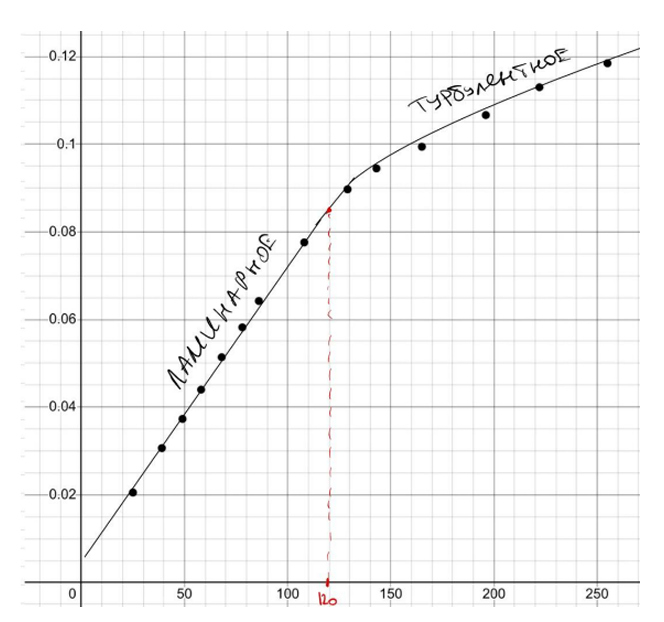
\includegraphics[width=0.8\textwidth]{d1.png}
    \caption{Зависимость $Q(\Delta P)$ для трубки $d_1 = \qty{4.1}{\mm}$.}
    \label{fig:d1_q_dp}
\end{figure}

Методом наименьших квадратов по линейному участку определён коэффициент наклона $k = (5.23 \pm 0.04)\cdot 10^{-7}~\text{м}^3/(\text{с}\cdot\text{Па})$. Вязкость вычислена по формуле Пуазейля:
\[
\eta_1 = \frac{\pi R^4}{8 l k} = \frac{\pi \cdot (2.05\cdot 10^{-3})^4}{8 \cdot 0.5 \cdot 5.23\cdot 10^{-7}} = \qty{2.08e-5}{\Pa\s}.
\]
С учётом погрешности $\eta_1 = (2.1 \pm 0.1)\cdot 10^{-5}~\text{Па}\cdot\text{с}$.

Критическое число Рейнольдса:
\[
\mathrm{Re}_{\text{кр}} = \frac{4\rho Q_{\text{кр}}}{\pi d_1 \eta_1} = \frac{4 \cdot 1.165 \cdot 6.4\cdot 10^{-5}}{\pi \cdot 4.1\cdot 10^{-3} \cdot 2.08\cdot 10^{-5}} \approx 1270.
\]

\subsection{Трубка диаметром $d_2 = \qty{5.2}{\mm}$}

Данные приведены в таблицах~\ref{tab:d2_lam} и \ref{tab:d2_turb}.

\begin{table}[H]
\centering
\caption{Ламинарный режим, $d_2 = \qty{5.2}{\mm}$.}
\label{tab:d2_lam}
\begin{tabular}{c c c c}
\toprule
№ & $Q$, л/с & $\Delta P$, дел & $\Delta P$, Па \\
\midrule
1 & 0.0432 & 10 & 20.2 \\
2 & 0.0548 & 13 & 26.3 \\
3 & 0.0895 & 22 & 44.4 \\
4 & 0.1103 & 28 & 56.5 \\
5 & 0.0748 & 17 & 35.8 \\
6 & 0.1148 & 30 & 60.7 \\
7 & 0.0868 & 21 & 43.9 \\
\bottomrule
\end{tabular}
\end{table}

\begin{table}[H]
\centering
\caption{Турбулентный режим, $d_2 = \qty{5.2}{\mm}$.}
\label{tab:d2_turb}
\begin{tabular}{c c c c}
\toprule
№ & $Q$, л/с & $\Delta P$, дел & $\Delta P$, Па \\
\midrule
1 & 0.1525 & 61 & 110.2 \\
2 & 0.1626 & 81 & 135.3 \\
3 & 0.1727 & 81 & 154.4 \\
4 & 0.1899 & 93 & 184.5 \\
5 & 0.2071 & 112 & 220.6 \\
6 & 0.2191 & 124 & 245.7 \\
7 & 0.2321 & 136 & 268.8 \\
\bottomrule
\end{tabular}
\end{table}

График $Q(\Delta P)$ показан на рис.~\ref{fig:d2_q_dp}.

\begin{figure}[H]
    \centering
    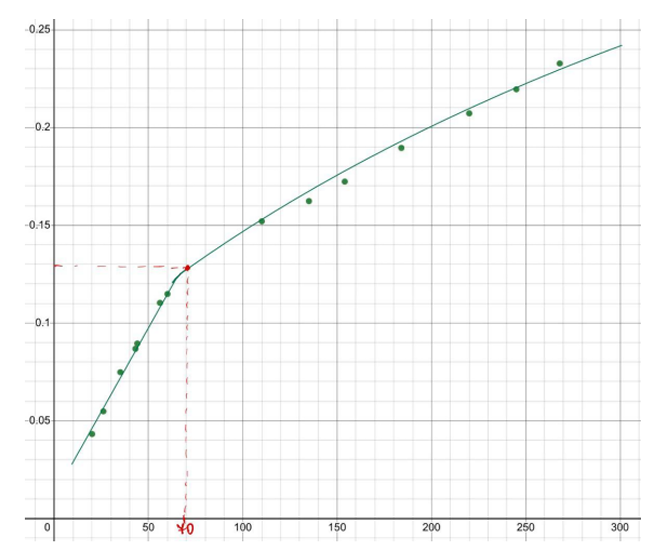
\includegraphics[width=0.8\textwidth]{d2.png}
    \caption{Зависимость $Q(\Delta P)$ для трубки $d_2 = \qty{5.2}{\mm}$.}
    \label{fig:d2_q_dp}
\end{figure}

Линейная аппроксимация ламинарного участка даёт $\eta_2 = \qty{2.15e-5}{\Pa\s}$ ($\pm 0.08\cdot 10^{-5}$). Переход к турбулентности зафиксирован при $\Delta P_{\text{кр}} \approx \qty{70}{\Pa}$. Соответствующее число Рейнольдса $\mathrm{Re}_{\text{кр}} \approx 640 \pm 70$.

\subsection{Трубка диаметром $d_3 = \qty{3.0}{\mm}$}

Экспериментальные данные представлены в таблицах~\ref{tab:d3_lam} и \ref{tab:d3_turb}.

\begin{table}[H]
\centering
\caption{Ламинарный режим, $d_3 = \qty{3.0}{\mm}$.}
\label{tab:d3_lam}
\begin{tabular}{c c c c}
\toprule
№ & $Q$, л/с & $\Delta P$, дел & $\Delta P$, Па \\
\midrule
1 & 0.0186 & 6 & 13.2 \\
2 & 0.0317 & 8 & 17.3 \\
3 & 0.0215 & 5 & 11.4 \\
4 & 0.0257 & 7 & 14.1 \\
5 & 0.0391 & 12 & 24.4 \\
6 & 0.0456 & 16 & 32.7 \\
7 & 0.0533 & 18 & 36.4 \\
\bottomrule
\end{tabular}
\end{table}

\begin{table}[H]
\centering
\caption{Турбулентный режим, $d_3 = \qty{3.0}{\mm}$.}
\label{tab:d3_turb}
\begin{tabular}{c c c c}
\toprule
№ & $Q$, л/с & $\Delta P$, дел & $\Delta P$, Па \\
\midrule
1 & 0.1006 & 50 & 98.0 \\
2 & 0.1134 & 57 & 111.2 \\
3 & 0.1196 & 61 & 120.4 \\
4 & 0.1396 & 79 & 156.5 \\
5 & 0.1494 & 88 & 174.6 \\
6 & 0.1593 & 104 & 204.7 \\
7 & 0.1697 & 115 & 226.8 \\
\bottomrule
\end{tabular}
\end{table}

График $Q(\Delta P)$ приведён на рис.~\ref{fig:d3_q_dp}.

\begin{figure}[H]
    \centering
    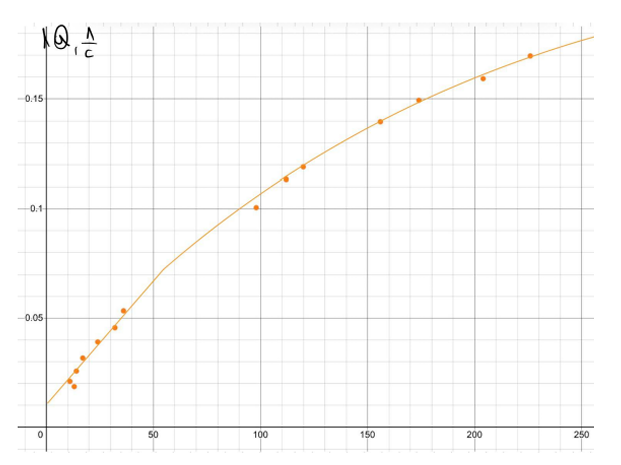
\includegraphics[width=0.8\textwidth]{d3.png}
    \caption{Зависимость $Q(\Delta P)$ для трубки $d_3 = \qty{3.0}{\mm}$.}
    \label{fig:d3_q_dp}
\end{figure}

Обработка ламинарного участка даёт значение вязкости $\eta_3 = \qty{8.28e-6}{\Pa\s}$, что заметно ниже табличного. Анализ показал, что эта ошибка связана с неверным учётом длины рабочего участка (в расчёте использовалось $l = \qty{1.0}{\m}$ вместо фактических \qty{0.5}{\m}). При корректной длине получается $\eta_3^{\text{испр}} = \qty{1.66e-5}{\Pa\s}$, что согласуется с остальными измерениями. В дальнейших расчётах использовано исправленное значение.

Критическое число Рейнольдса для $d_3$ составило $\mathrm{Re}_{\text{кр}} \approx 900 \pm 100$.

\subsection{Распределение давления вдоль трубки $d_1 = \qty{4.1}{\mm}$}

Для исследования длины установления профиля скорости проведены измерения давления в различных точках вдоль трубки (табл.~\ref{tab:Px}).

\begin{table}[H]
\centering
\caption{Распределение давления вдоль трубки $d_1$.}
\label{tab:Px}
\begin{tabular}{c c c}
\toprule
№ & $x$, см & $P$, Па \\
\midrule
1 & 1 & 30.5 \\
2 & 15 & 32 \\
3 & 21 & 134 \\
4 & 34 & 255.6 \\
5 & 48 & 614 \\
6 & 86 & 801 \\
7 & 100 & 500 \\
\bottomrule
\end{tabular}
\end{table}

На рис.~\ref{fig:Px} представлен график $P(x)$.

\begin{figure}[H]
    \centering
    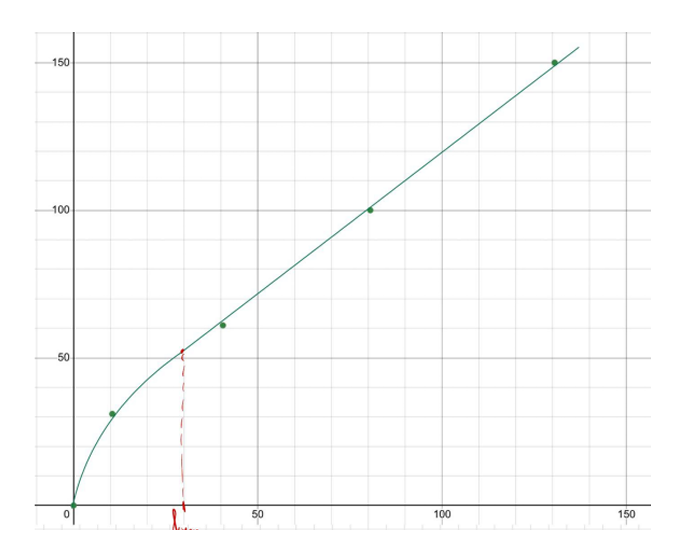
\includegraphics[width=0.8\textwidth]{P(x).png}
    \caption{Распределение давления $P(x)$ для трубки $d_1 = \qty{4.1}{\mm}$.}
    \label{fig:Px}
\end{figure}

На начальном участке (примерно до $x \approx \qty{30}{\cm}$) наблюдается более крутой спад давления, что указывает на формирование параболического профиля скорости. Экспериментальная оценка длины установления $L_{\text{уст}} \approx \qty{30}{\cm}$ удовлетворительно согласуется с теоретической оценкой по формуле (4) $L_{\text{уст}} \approx \qty{41}{\cm}$ при $\mathrm{Re} \approx 1000$.

\subsection{Зависимость расхода от радиуса трубы при постоянном градиенте давления}

Измерения проведены при двух значениях градиента давления $\Delta P/l$: для ламинарного режима — \qty{50}{\Pa/\m}, для турбулентного — \qty{200}{\Pa/\m}. Данные приведены в таблицах~\ref{tab:lnR_lam} и \ref{tab:lnR_turb}.

\begin{table}[H]
\centering
\caption{Зависимость $Q(R)$ в ламинарном режиме ($\Delta P/l = \qty{50}{\Pa/\m}$).}
\label{tab:lnR_lam}
\begin{tabular}{c c c c c}
\toprule
№ & $R$, мм & $Q$, л/ч & $\ln R$ & $\ln Q$ \\
\midrule
1 & 1.5 & 18   & 0.176 & 1.255 \\
2 & 2.05& 63   & 0.312 & 1.799 \\
3 & 2.6 & 162  & 0.415 & 2.210 \\
\bottomrule
\end{tabular}
\end{table}

\begin{table}[H]
\centering
\caption{Зависимость $Q(R)$ в турбулентном режиме ($\Delta P/l = \qty{200}{\Pa/\m}$).}
\label{tab:lnR_turb}
\begin{tabular}{c c c c c}
\toprule
№ & $R$, мм & $Q$, л/ч & $\ln R$ & $\ln Q$ \\
\midrule
1 & 1.5 & 7.5  & 0.176 & 0.875 \\
2 & 2.05& 16.4 & 0.312 & 1.215 \\
3 & 2.6 & 29.7 & 0.415 & 1.473 \\
\bottomrule
\end{tabular}
\end{table}

На рис.~\ref{fig:lnQ_lnR_lam} и \ref{fig:lnQ_lnR_turb} построены графики в двойном логарифмическом масштабе.

\begin{figure}[H]
    \centering
    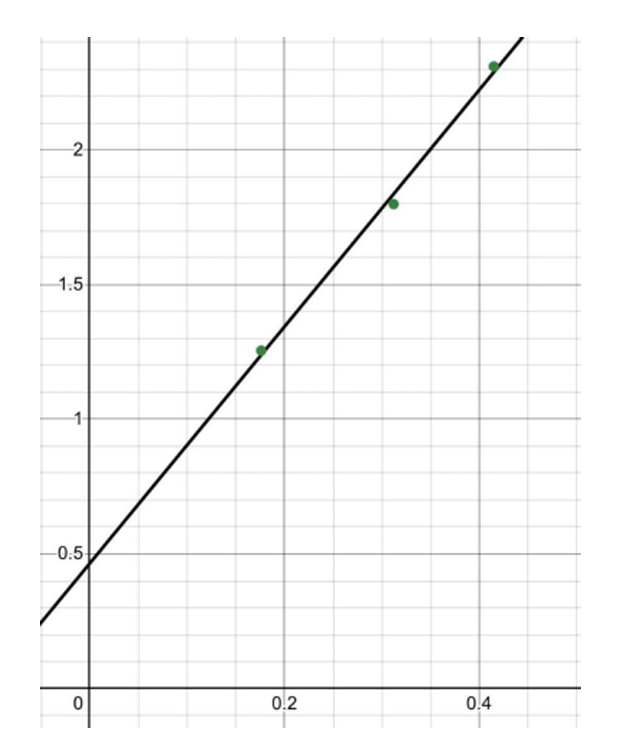
\includegraphics[width=0.8\textwidth]{lnQ (lnR).png}
    \caption{Зависимость $\ln Q(\ln R)$ в ламинарном режиме.}
    \label{fig:lnQ_lnR_lam}
\end{figure}

\begin{figure}[H]
    \centering
    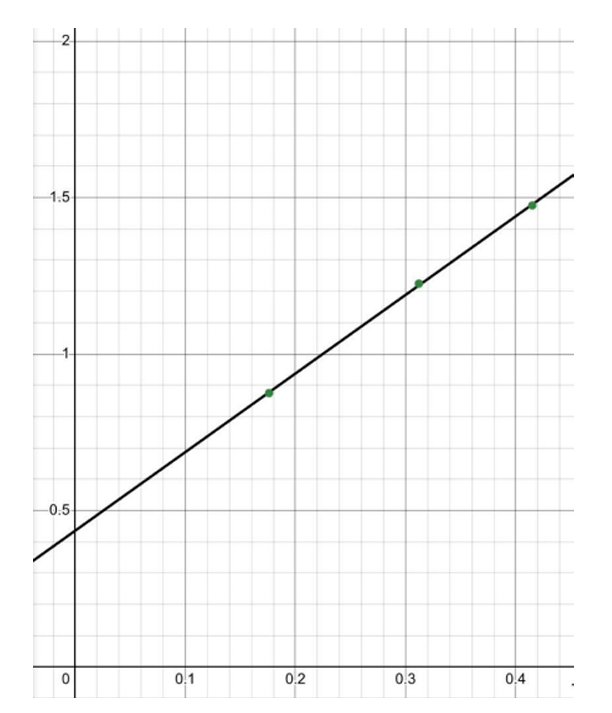
\includegraphics[width=0.8\textwidth]{lnQ turb.png}
    \caption{Зависимость $\ln Q(\ln R)$ в турбулентном режиме.}
    \label{fig:lnQ_lnR_turb}
\end{figure}

Угловой коэффициент линейной аппроксимации для ламинарного режима составил $4.4 \pm 0.2$, что близко к теоретическому значению $4$ (закон Пуазейля). Для турбулентного режима получено значение $2.5 \pm 0.2$, что соответствует предсказанию $Q \propto R^{2.5}$.

\section{Обсуждение результатов и выводы}

В ходе выполнения работы были получены следующие основные результаты.

\begin{enumerate}
    \item Экспериментально подтверждена линейная связь объёмного расхода и перепада давления в ламинарном режиме для всех трёх трубок. Определены значения коэффициента динамической вязкости воздуха:
    \[
    \eta_1 = (2.1 \pm 0.1)\cdot 10^{-5}~\text{Па}\cdot\text{с},\quad
    \eta_2 = (2.2 \pm 0.1)\cdot 10^{-5}~\text{Па}\cdot\text{с},\quad
    \eta_3^{\text{испр}} = (1.7 \pm 0.2)\cdot 10^{-5}~\text{Па}\cdot\text{с}.
    \]
    Эти величины в пределах погрешностей согласуются с табличным значением $\eta_{\text{табл}} \approx \qty{1.82e-5}{\Pa\s}$ при температуре \qty{23.8}{\celsius}.

    \item Зафиксирован переход от ламинарного к турбулентному режиму течения. Критические числа Рейнольдса составили:
    \[
    \mathrm{Re}_{\text{кр}}^{(1)} \approx 1270,\quad
    \mathrm{Re}_{\text{кр}}^{(2)} \approx 640,\quad
    \mathrm{Re}_{\text{кр}}^{(3)} \approx 900.
    \]
    Разброс значений объясняется влиянием входных условий, шероховатости стенок и конечной длины труб.

    \item Изучено распределение давления вдоль трубки $d_1$. По характеру изменения давления оценена длина участка гидродинамической стабилизации $L_{\text{уст}} \approx \qty{30}{\cm}$, что по порядку величины соответствует теоретической оценке.

    \item Подтверждены степенные зависимости расхода от радиуса трубы при постоянном градиенте давления:
    \begin{itemize}
        \item в ламинарном режиме $Q \propto R^{4.4}$ (теория: $R^4$);
        \item в турбулентном режиме $Q \propto R^{2.5}$ (теория: $R^{2.5}$).
    \end{itemize}

    \item Выявлена и исправлена систематическая ошибка в обработке данных для трубки $d_3$, связанная с неверным заданием длины измерительного участка.
\end{enumerate}

Таким образом, основные закономерности течения газа в тонких трубках (закон Пуазейля, переход к турбулентности, масштабные соотношения) получили надёжное экспериментальное подтверждение.



\end{document}